% !TEX encoding = UTF-8 Unicode
% -*- coding: UTF-8; -*-
% vim: set fenc=utf-8
\documentclass[a4paper,12pt,french]{article}

\usepackage{centrale}
\usepackage{algorithm}
\usepackage{algorithmic}

\hypersetup{
    pdftitle={Parareal Algorithm},
    pdfauthor={Oussama BOUHENNICHE},
    pdfsubject={Parareal Algorithm},
    pdfproducer={Conversion PDF à insérer},
    pdfkeywords={Parareal, euler, runge kutta, scipy.integrate, lorenz system} %
}

\DeclareGraphicsRule{.ai}{pdf}{.ai}{.png} % pour insérer des documents .ai
\graphicspath{ {./img/}} % pour ne pas avoir à ajouter eps/ton-image.jpg

% ------------- Packages spéciaux, nécessaires pour ce rapport, à insérer ici ------------- 


\begin{document}

% --------------------------------------------------------------
%                       Page de garde
% --------------------------------------------------------------

\begin{titlepage}
\begin{center}

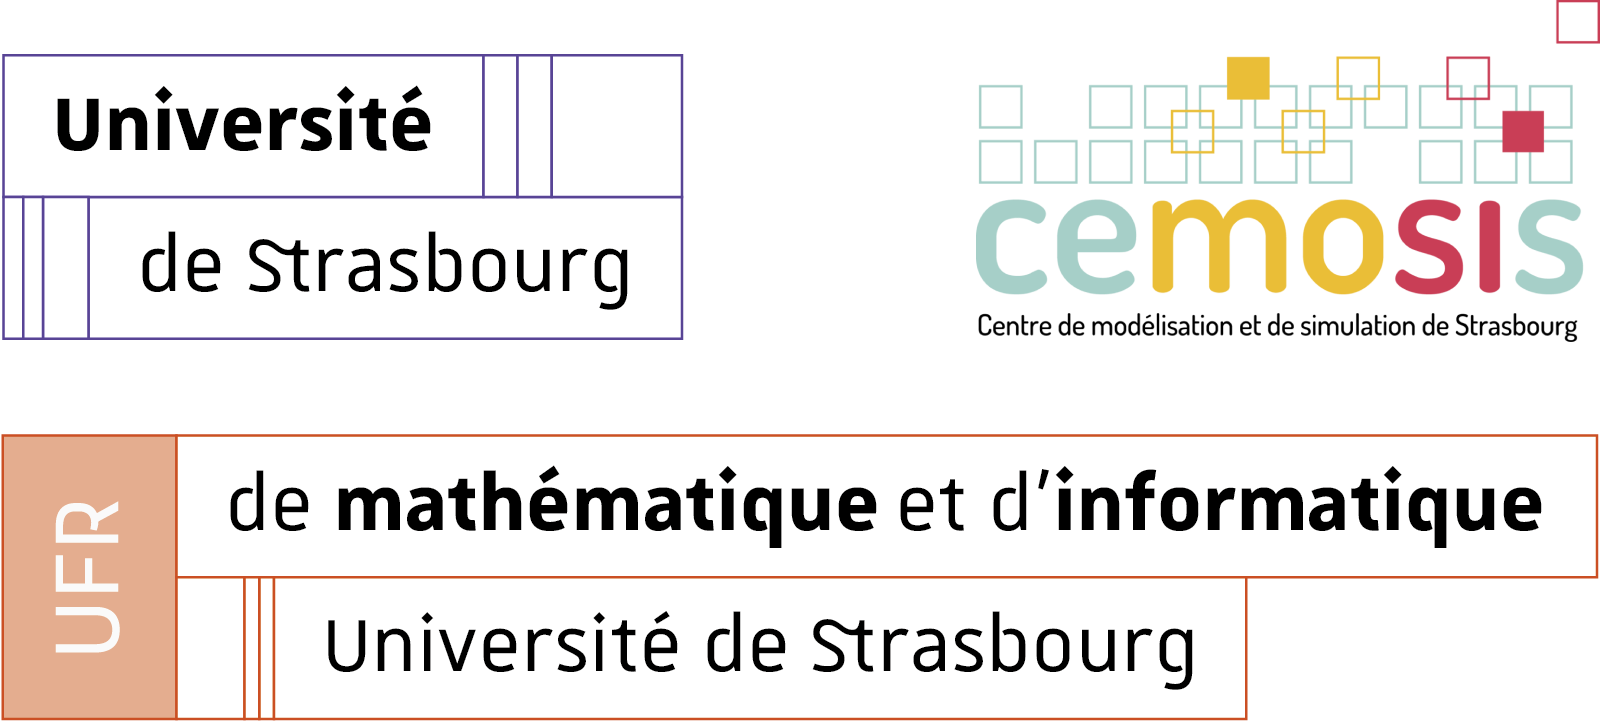
\includegraphics[width=1\textwidth]{logo.png}\\[1cm]

{\large Master 1 CSMI : Scientific Computation and Mathematics of Innovation}\\[0.5cm]

% Title
\rule{\linewidth}{0.5mm} \\[0.4cm]
{ \huge \bfseries Parareal Algorithm \\[0.4cm] }
\rule{\linewidth}{0.5mm} \\[1.5cm]

% Author and supervisor
\noindent
\begin{minipage}{0.6\textwidth}
  \begin{flushleft} \large
    \emph{Authors :}\\
    Oussama \textsc{BOUEHNNICHE}\\
    Narimane \textsc{ZAOUACHE}
  \end{flushleft}
\end{minipage}%
\begin{minipage}{0.4\textwidth}
  \begin{flushright} \large
    \emph{Supervisors :} \\
    M.~Christophe \textsc{Prud'homme}
  \end{flushright}
\end{minipage}

\vfill

% Bottom of the page
{\today}

\end{center}
\end{titlepage}

% --------------------------------------------------------------
%                            Abstract
% --------------------------------------------------------------
\newpage
\thispagestyle{empty}

\vspace*{\fill}
\noindent\rule[2pt]{\textwidth}{0.5pt}\\
{\textbf{Abstract :}}
Solving time-dependent ordinary differential equations (ODEs) and partial differential equations (PDEs) numerically is 
    a significant task in computational domains. Traditional methods can be time-consuming, especially for long simulation or complex systems.
    
    The Parareal algorithm offers an efficient parallel solution to accelerate ODEs and PDEs solving.
    
    In this project, we aim to study and implement the Parareal algorithm in sequentially and in parallel and test it on lorenz system\\

{\noindent\textbf{keywords :}}
Parareal, Euler, Runge kutta, Scipy.integrate, Lorenz system
\\
\noindent\rule[2pt]{\textwidth}{0.5pt}

\vspace*{\fill}
\newpage

% --------------------------------------------------------------
%                    Table des matières 
% --------------------------------------------------------------

\thispagestyle{empty}
\tableofcontents
%\newpage

% --------------------------------------------------------------
%                         Début du corps
% --------------------------------------------------------------
\newpage
\section{Introduction}
This project, carried out by \href{http://cemosis.fr}{Cemosis} \cite{cemosis} (Centre for Modeling and Simulation in Strasbourg), focuses on the study and implementation of the Parareal algorithm \cite{lions2001resolution}, a parallel method for temporal discretization.\\

The primary objective of this project is to study the Parareal algorithm and its application in solving time-dependent ordinary differential equations (ODEs) (And for future prespective, solving partial differential equations (PDEs) ), while also examining commonly used numerical methods for solving the Lorenz system, such as Euler's method, the Runge-Kutta method, and the scipy.integrate functions. \\

The project is divided into four sub-objectives:
\begin{enumerate}
    \item Study lorenz system and Implement Lorenz Model, also study different ODEs solvers and its implementation.
    \item Explore the scipy.integrate package for ODEs solving and test it on lorenz system.
    \item Study the Parareal algorithm and implement it in sequential.
    \item study the parallelisation mechanism of the Parareal algorithm and implement it.
\end{enumerate} \\

Throughout this project, we will utilize Python as the programming language, scipy.integrate package and mpi4py for parallelisation. By exploring the Parareal algorithm and its implementation in different configurations, we aim to demonstrate its potential in accelerating the solution of ODEs and its applicability to large-scale simulations.


% --------------------------------------------------------------
%                         Partie 1
% --------------------------------------------------------------

\newpage
\section{The Lorenz system}
\subsection{Background}


The Lorenz system\cite{lorenz1963deterministic}, introduced by meteorologist Edward Lorenz in 1963, is a set of nonlinear ordinary differential equations describing the behavior of a dynamic system. 

This system is used as a mathematical model to study phenomena such as convection and turbulence, as well as in other areas such as population dynamics, chaos theory, and control theory.

\subsection{Equations Model}

The Lorenz system it can be described by the following three equations:

\begin{equation}
\large
\begin{cases}
    \displaystyle\frac{dx}{dt} = \sigma(y - x) \\
    \displaystyle\frac{dy}{dt} = x(\rho - z) - y \\
    \displaystyle\frac{dz}{dt} = xy - \beta z
\end{cases}
\normalsize
\end{equation}\\
   
where:
\begin{itemize}
    \item $x$ is the rate of convective overturning,
    \item $y$ is the horizontal temperature variation,
    \item $z$ is the vertical temperature variation,
    \item $\sigma$ is the Prandtl number,
    \item $\rho$ is the Rayleigh number,
    \item $\beta$ is a geometrical factor.
\end{itemize}

The equations describe the behavior of a two-dimensional fluid layer that is heated uniformly from below and cooled from above.\\
   
For the parameter values $\sigma = 10$, $b = 8/3$, and $\rho = 28$, a large set of solutions are attracted to a butterfly shaped set (called the Lorenz attractor). \\

The trajectory seems to randomly jump betwen the two wings of the butterfly (see figure\reff{fig:1}). 
   
\begin{figure}[ht!]
    \centering
    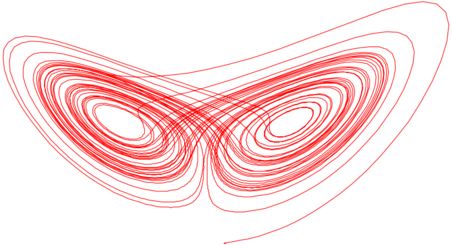
\includegraphics[width=0.5\textwidth]{img/lorenz-attractor-112761.png}
    \caption{Lorenz attractor.}
    \label{fig:1}
\end{figure}

The numerical solution of the Lorenz system involves using numerical methods to approximate the trajectory of the state variables over time. 

%\begin{listing}[ht]
%\inputminted[mathescape,
               %numbersep=5pt,
               %gobble=2,
               %frame=lines,
               %framesep=2mm]{python}{code/}
%\caption{Du code informatique}
%\label{listing:id-du-code}
%\end{listing}


% --------------------------------------------------------------
%                            Partie 2
% --------------------------------------------------------------

\section{ODEs solvers}
\subsection{Euler Methods}
Euler methods \cite{lakoba2012simple} are numerical techniques used to approximate solutions to ordinary differential equations (ODEs). There are two main variants: the explicit Euler method and the implicit (backward) Euler method.
\subsubsection{Explicit Euler Method}
The explicit Euler method is the simplest and most straightforward technique for solving ODEs. Given an initial value problem of the form:

\[
\frac{dy}{dt} = f(t, y), \quad y(t_0) = y_0,
\]

the explicit Euler method approximates the solution at discrete time steps. If \(h\) is the step size, the method uses the following update rule:

\[
y_{n+1} = y_n + h f(t_n, y_n).
\]

This formula is derived from the Taylor series expansion and provides a first-order accurate approximation. It is called "explicit" because it explicitly computes the next value \(y_{n+1}\) using the current value \(y_n\).

The stability of the explicit Euler method depends on the step size \(h\) and the properties of the function \(f(t, y)\).

For a simple linear test equation of the form:

\[
\frac{dy}{dt} = \lambda y,
\]

where \(\lambda\) is a constant, the explicit Euler update rule becomes:

\[
y_{n+1} = y_n + h \lambda y_n = (1 + h \lambda) y_n.
\]

The method is stable if the magnitude of the factor \(1 + h \lambda\) is less than or equal to 1. This implies:

\[
|1 + h \lambda| \leq 1.
\]

For \(\lambda\) with a negative real part, this condition requires the step size \(h\) to be very small. If \(h\) is too large, the method can become unstable, leading to exponentially growing errors.

\subsubsection{Implicit (Backward) Euler Method}
The implicit or backward Euler method is another technique for solving ODEs, and it is particularly useful for stiff equations. The method is given by:

\[
y_{n+1} = y_n + h f(t_{n+1}, y_{n+1}),
\]

where \(y_{n+1}\) is implicitly defined. This means that \(y_{n+1}\) appears on both sides of the equation, making it necessary to solve an equation to find \(y_{n+1}\). This method is generally more stable than the explicit Euler method.

For the same test equation, the implicit Euler update rule becomes:

\[
y_{n+1} = y_n + h \lambda y_{n+1}.
\]

Rearranging gives:

\[
y_{n+1} = \frac{y_n}{1 - h \lambda}.
\]

The method is stable if the magnitude of the factor \( \frac{1}{1 - h \lambda} \) is less than or equal to 1. This implies:

\[
\left| \frac{1}{1 - h \lambda} \right| \leq 1.
\]

For \(\lambda\) with a negative real part, this condition is satisfied for any step size \(h > 0\). Therefore, the implicit Euler method is unconditionally stable for linear problems with \(\lambda\) having a negative real part. This makes it particularly suitable for stiff problems, where large step sizes can be used without losing stability.

\subsubsection*{Comparison}

\begin{itemize}
    \item \textbf{Stability}: The implicit Euler method is more stable than the explicit Euler method.
    \item \textbf{Computational Effort}: The explicit Euler method is simpler and requires less computational effort per step since it does not require solving an equation. The implicit Euler method requires solving a (typically nonlinear) equation at each step, which can be computationally intensive.
    \item \textbf{Accuracy}: Both methods are first-order accurate, meaning the error per step is proportional to the step size \(h\).
\end{itemize}

\subsection{Runge-Kutta Methods}

The Runge-Kutta method \cite{butcher1996history} is a family of numerical techniques used to approximate solutions to ordinary differential equations (ODEs). It is more accurate and versatile than the Euler methods and is widely used in scientific computing.\\

The basic idea behind the Runge-Kutta method is to use weighted averages of function evaluations at multiple points within each time step to improve accuracy. The most commonly used variant is the fourth-order Runge-Kutta method (RK4), which uses four function evaluations per step.

\subsubsection{Fourth-Order Runge-Kutta (RK4)}

Given an initial value problem of the form:

\[
\frac{dy}{dt} = f(t, y), \quad y(t_0) = y_0,
\]

and a step size \(h\), the RK4 method updates the solution as follows:

\begin{align*}
k_1 &= h f(t_n, y_n), \\
k_2 &= h f(t_n + \frac{h}{2}, y_n + \frac{k_1}{2}), \\
k_3 &= h f(t_n + \frac{h}{2}, y_n + \frac{k_2}{2}), \\
k_4 &= h f(t_n + h, y_n + k_3), \\
y_{n+1} &= y_n + \frac{1}{6}(k_1 + 2k_2 + 2k_3 + k_4).
\end{align*}

Here, \(k_1\), \(k_2\), \(k_3\), and \(k_4\) are intermediate values computed at different points within the time step. The final solution \(y_{n+1}\) is a weighted average of these intermediate values.\\

The RK4 method is a fourth-order accurate method, meaning that the error per step is proportional to \(h^4\). This makes it significantly more accurate than first-order methods like the Euler methods. RK4 is widely used in practice due to its balance between accuracy and computational efficiency.

\begin{itemize}
    \item \textbf{Accuracy}: RK4 provides higher accuracy compared to first-order methods like the Euler methods and is suitable for a wide range of ODEs.
    \item \textbf{Efficiency}: Although more computationally intensive than first-order methods, RK4 strikes a good balance between accuracy and computational effort.
\end{itemize}

%\subsubsection*{Implementation}
%We implement the RK2 (see \reff{fig:2}) and RK4 (see %\reff{fig:3}) method in python.
%
%   
%\begin{figure}[ht!]
%    \centering
%    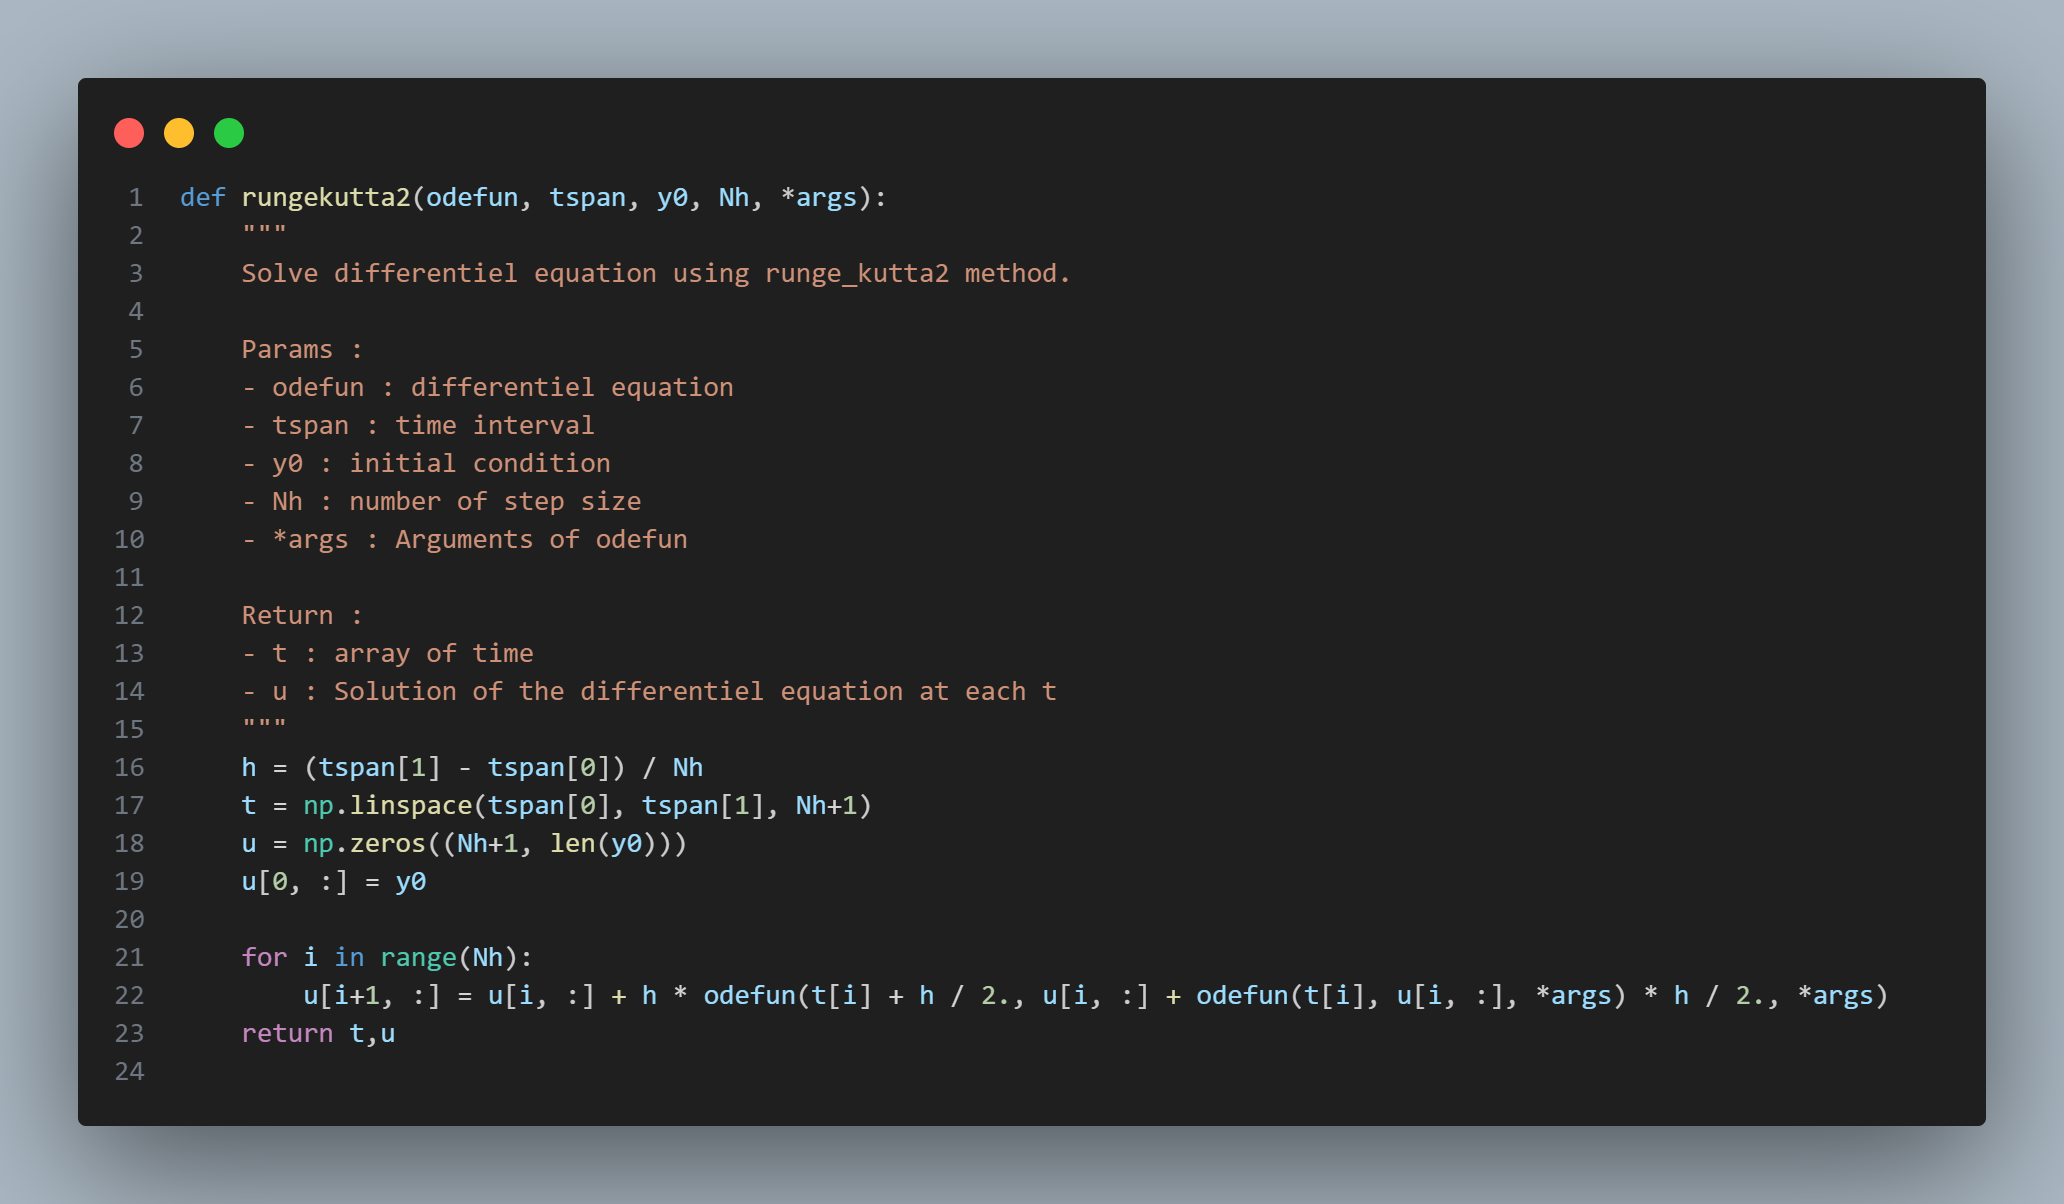
\includegraphics[width=0.78\textwidth]{img/rk2.png}
%    \caption{RK2}
%    \label{fig:2}
%\end{figure}
%
%   
%\begin{figure}[ht!]
%    \centering
%    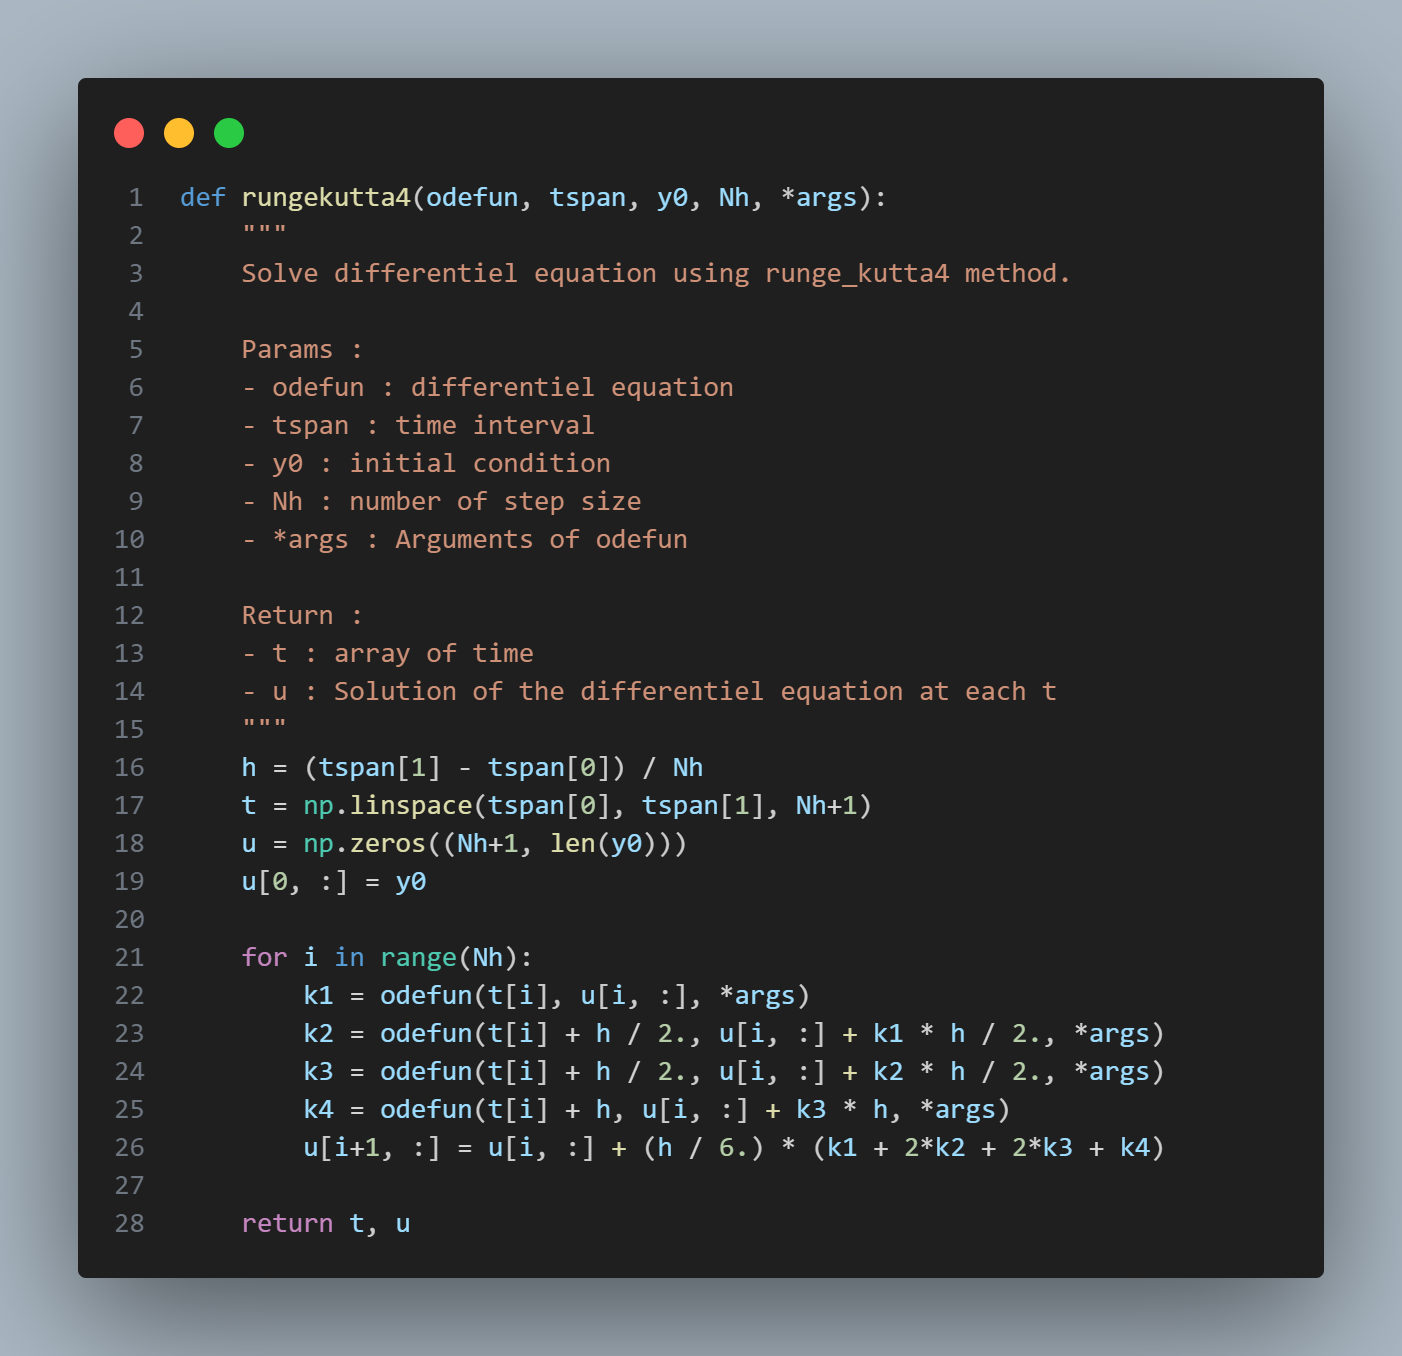
\includegraphics[width=0.78\textwidth]{img/rk4.png}
%    \caption{RK4}
%    \label{fig:3}
%\end{figure}
%\newpage


\subsubsection{Adaptive Step-Size Runge-Kutta Method}

The Runge-Kutta method can be extended to include adaptive step-size control. In adaptive step-size RK4, the step size \(h\) is adjusted dynamically based on the local error estimate obtained during each integration step. By comparing the local error to a specified tolerance, the method adapts the step size to ensure accurate integration while minimizing computational cost.

\subsubsection*{Algorithm}

The adaptive RK4 algorithm involves the following steps:

\begin{enumerate}
    \item Start with an initial step size \(h_0\) and specify a tolerance \(tol\).
    \item At each step, perform two RK4 integration steps: one with step size \(h\) and another with step size \(h/2\).
    \item Compute the difference between the solutions obtained with the two step sizes to estimate the local error.
    \item If the error is within the tolerance, accept the solution and proceed to the next step. Otherwise, adjust the step size based on the error estimate.
    \item Repeat the process until reaching the desired endpoint.
\end{enumerate}

\subsubsection*{Step Size Adjustment}

The step size adjustment in adaptive RK4 is typically based on the estimated local error. Common strategies include:

\begin{itemize}
    \item If the error is smaller than the tolerance, increase the step size to take larger steps.
    \item If the error exceeds the tolerance, decrease the step size to take smaller steps.
    \item The step size adjustment factor can be chosen based on empirical rules or adaptive strategies to balance accuracy and efficiency.
\end{itemize}

The Adaptive RK4 method provides high accuracy and automatically adjusts the step size to minimize computational cost while ensuring accurate integration.

\subsection{SciPy.integrate Package}
The Scipy.integrate \cite{SciPy} is a sub-library of SciPy offers functions such as \texttt{odeint} and \texttt{solve\_ivp} for solving ODEs, as well as other methods for single and multiple function integration.

\subsubsection{odeint from scipy.integrate}

The \texttt{odeint} function from \texttt{scipy.integrate} is widely used for numerically solving systems of ordinary differential equations (ODEs) with initial conditions \cite{scipy_ode}. It uses the LSODA \cite{hindmarsh2005lsoda} (Livermore Solver for Ordinary Differential Equations) algorithm to perform integration, thus providing a fast and efficient solution. Although simple to use, \texttt{odeint} is limited in terms of control over integration methods and does not allow for the specification of events or constraints.
\subsubsection{solve\_ivp}

The \texttt{solve\_ivp} function from \texttt{scipy.integrate} offers a more unified and flexible interface for solving ODEs. It supports a variety of integration methods, including RK45 and RK23, and also allows for the specification of events and constraints for flexible termination conditions. \texttt{solve\_ivp} is thus more versatile than \texttt{odeint}, providing increased control over the integration process and suitable for a wider variety of ODE problems.\\

Overall, \texttt{scipy.integrate} from SciPy offers powerful tools for solving a variety of numerical integration problems, especially ODEs. While \texttt{odeint} is simple to use and fast for common cases, \texttt{solve\_ivp} offers finer flexibility and control, making it suitable for a broader range of problems. The choice between these two functionalities will depend on the specific requirements of the problem at hand.

\section{Parareal}
The Parareal algorithm is a parallel-in-time integration method designed to solve large-scale time-dependent differential equations. It was introduced by Lions, Maday, and Turinici in 2001 \cite{lions2001resolution}. The method aims to address the challenge of efficiently solving these equations, which is often computationally expensive, by parallelizing the time dimensions.

Parareal is a  designed to tackle initial value problems (IVPs \cite{shampine2000initial}), which are a class of mathematical problems where we aim to find a function satisfying a differential equation, given an initial condition. These problems arise frequently in various scientific and engineering disciplines, modeling phenomena like motion, heat transfer, and population growth.

Traditionally, solving IVPs involves sequential computations, meaning calculations proceed one step at a time. While effective, this approach can be time-consuming for complex problems, especially when dealing with large time intervals. Parareal offers an alternative by leveraging parallelism

\subsection{The Core Idea of Parareal}
Parareal breaks down the solution process into two parts:
\begin{itemize}
    \item \textbf{Coarse Integrator:} This is a computationally cheap and fast method that provides an approximate solution across the entire time interval.
    \item \textbf{Fine Integrator:} This is a more accurate but computationally expensive method used to refine the solution on smaller time intervals.
\end{itemize}

The key innovation lies in using both integrators iteratively. The coarse solution provides a starting point for the fine integrator on smaller subintervals. The corrections obtained from the fine integrator are then used to improve the coarse solution. This interplay between the two integrators allows for parallel computations, significantly speeding up the solution process.

\subsection{How it Works}
\subsubsection*{Initialisation}
\begin{itemize}
    \item {\textbf{Define the Solvers:}
            \begin{itemize}
                \item \textbf{Coarse Solver ($G$):} Provides quick but less accurate approximations.
                    
                \item \textbf{Fine Solver ($F$):} Provides accurate solutions but is computationally expensive.
            \end{itemize}}

    \item \textbf{Decompose the Time Interval:} Divide the total time interval $[t_0,T]$ into $N$ equal subintervals, each of length $\Delta T$. 
\end{itemize}

\subsubsection*{Zero Iteration}
   Use the coarse solver $G$ serially to obtain an initial approximation of the solution:
    $$ U_{j+1}^0 = G(t_j,t_{j+1}, U_j^0)   \;\;\;\;\;\;\;\; j = 0, ..., N-1$$.
\subsubsection*{Subsequent Iterations} 
Update the solution values using a combination of the coarse and fine solvers:
    $$ U_{j+1}^k = G(t_j,t_{j+1},U_j^k) + F(t_j,t_{j+1},U_j^{k-1}) -G(t_j,t_{j+1},U_j^{k-1}) \;\;\;\;\;\;\;\; j = 0, ... ,N-1$$.
\subsubsection*{Convergence Check}
        Verify convergence by checking the difference between successive iterations:
      $$   | U_j^k - U_j^{k-1} | < \epsilon $$
   where $ \epsilon $ is a predefined tolerance. 

\begin{algorithm}
\caption{Parareal Algorithm}
\begin{algorithmic}[1]
\STATE \textbf{Given:} Coarse function $G$, fine function $F$, number of time steps $N$, maximum number of iterations $K$, $\epsilon$ tolerance.
\STATE \textbf{Initialize:} \begin{itemize}
    \item  $U_0^0 = u_0$,
    \item $ U_{j+1}^0 = G(t_j,t_{j+1}, U_j^0) \;\;\;j = 0,1, \ldots, N-1$
\end{itemize}
\WHILE{$|U^k-U^{k-1}| > \epsilon $}
    \begin{itemize}
        \item  $ U_{j+1}^k = G(t_j,t_{j+1},U_j^k) + F(t_j,t_{j+1},U_j^{k-1}) -G(t_j,t_{j+1},U_j^{k-1})\;\;\;\;\;\;\;\;\;\;\newline j = 0,1, ... ,N-1$.
    \end{itemize}
\ENDWHILE
\STATE \textbf{Return:} $U^k$
\end{algorithmic}
\end{algorithm}

\subsection{Stability of Parareal}
The stability of the Parareal algorithm is influenced by the interplay between the coarse and fine solvers, the time step sizes, and the iterative process. Careful selection and tuning of these components are essential to ensure stable and accurate solutions.
\begin{itemize}
    \item \textbf{Choice of Solvers:} The stability properties of both the coarse and fine solvers directly impact the overall stability of the Parareal algorithm. Ideally, the coarse solver should be stable and provide a good approximation to prevent error amplification.
    \item \textbf{Time Step Sizes:} The size of the time steps for both the coarse and fine solvers can affect stability. If the coarse solver uses a much larger time step than the fine solver, it may introduce significant errors that could destabilize the algorithm.
    \item \textbf{Number of Iterations:} The algorithm iterates until convergence is achieved. The rate of convergence can influence stability; rapid convergence is desirable but not at the expense of stability. 
\end{itemize}
\newpage
\subsection{Parallelization}
The Parareal algorithm is designed to exploit parallelism in time integration, allowing different time intervals to be processed simultaneously. This capability can significantly speed up the solution of time-dependent problems, particularly when dealing with large-scale simulations. 
Here’s an overview of how the Parareal algorithm achieves parallelization:
\begin{enumerate}
    \item \textbf{Time Decomposition:} Divide the total time interval \([0, T]\) into \(N\) sub-intervals: \([T_0, T_1], [T_1, T_2], ..., [T_{N-1}, T_N]\). Each sub-interval can be processed independently once the initial conditions are known.
    \item \textbf{Coarse Propagation:} Use a coarse solver \(G\) to compute an initial guess of the solution over the entire time domain. This step is sequential but relatively quick due to the use of a coarse solver with larger time steps.
    \item \textbf{Parallel Fine Propagation:} Solve the problem over each sub-interval using a fine solver \(F\) in parallel. The fine solver provides a more accurate solution but operates within smaller time steps, confined to the sub-intervals.
    \item \textbf{Iterative Correction:} Iterate to improve the solution by combining the coarse and fine solutions. Each iteration corrects the previous iteration's solution using the fine solver's results. This step involves communication and synchronization among processors to update the initial conditions for the next iteration.
\end{enumerate}


\begin{algorithm}
\caption{Parareal Algorithm (parallel version)} 
\begin{algorithmic}[1]
\STATE \textbf{Given:} Coarse function $G$, fine function $F$, number of time steps $N$, maximum number of iterations $K$, $\epsilon$ tolerance, number of process.
\STATE \textbf{Initialize: in sequential} \begin{itemize}
    \item  $U_0^0 = u_0$,
    \item $ U_{j+1}^0 = G(t_j,t_{j+1}, U_j^0) \;\;\;j = 0,1, \ldots, N-1$
\end{itemize}
\WHILE{$|U^k-U^{k-1}| > \epsilon $}
    \begin{itemize}
        \item run the fine solver on each process and given a sub-interval of the time slices, in parallel: $F(t_j,t_{j+1}, U_j^{k-1}) \;\;\;\;\;\;\;\;\;\; j = 0,1, ... ,N-1$.
        \item  communicate fine solution and update u in sequetial and share it to all process: $\;\;\;\;\;\;\;\;\; j = 0,1, ... ,N-1$.
        \newline
        $ U_{j+1}^k = G(t_j,t_{j+1},U_j^k) + F(t_j,t_{j+1},U_j^{k-1}) -G(t_j,t_{j+1},U_j^{k-1})$
    \end{itemize}
\ENDWHILE
\STATE \textbf{Return:} $U^k$
\end{algorithmic}
\end{algorithm}
\newpage
\subsubsection*{Implementaion requirment}
It require for using a dedicated framework for parallelisation including Message passing(for exchanging information between processors to synchronize computations and compute corrections) and shared-memory or distributed-memory parallelism(Utilizing shared-memory systems with threads or distributed-memory systems with message passing interfaces) like \textbf{MPI} \cite{forum1994mpi} or \textbf{OpenCL} \cite{munshi2011opencl}.

\newpage
\section{Implementation}
In this section, we will outline the implementation details of our solution and describe the project's structure.

Our implementation was done in Python, utilizing libraries like NumPy for numerical operations, SciPy for scientific computing, and Matplotlib for plotting results. The parallel implementation of the Parareal algorithm was facilitated by the mpi4py library.

\subsection{Project Structure}
The project is available on  \href{https://github.com/master-csmi/2024-m1-parareal}{github} and is structured as shown in the picture below \reff{fig:7}:
\begin{figure}[ht!]
    \centering
    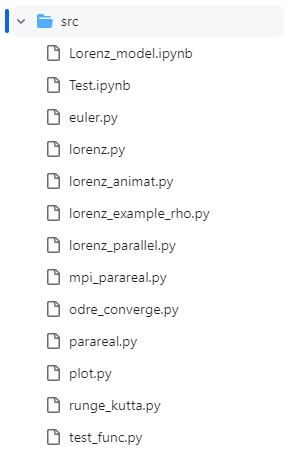
\includegraphics[width=0.5\textwidth]{img/code_struct.jpg}
    \caption{Code structure}
    \label{fig:7}
\end{figure}
\newline

\begin{itemize}
    \item \textbf{Lorenz\_model.ipynb:} contains a testing solution of lorenz system solved by our ODEs solvers and some testing scenarios of parareal.
    \item \textbf{Test.ipynb} contains a testing solution of our tests functions solved by our ODEs solvers and parareal.
    \item \textbf{euler.py:} contains the implementation of euler methods ( cours tan \cite{CoursTan}).
    \item \textbf{lorenz.py:} contains the differentail equation sytem of lorenz
    \item \textbf{lorenz\_animat.py:} contains 
    \item \textbf{lorenz\_example\_rho.py:} contains a testing solutions of the Lorenz system for different values of rho.
    \item \textbf{lorenz\_parallel.py:} contains a testing solution of lorenz system solved by parareal algorithm in parallel.
    \item \textbf{mpi\_parareal.py:} contains the implementation of parareal algorithm in parallel.
    \item \textbf{odre\_converge.py:} contains a testing of influence of Solver Choice on Parareal Convergence Order.
    \item \textbf{parareal.py:} contains the implementation of parareal algorithm in sequential.
    \item \textbf{plot.py:} contains a plot function for 3d plot.
    \item \textbf{runge\_kutta.py:} contains the implementation runge kutta methods (rk4, rk2, and adaptative time stepping rk4).
    \item \textbf{test\_func.py:} contains a simple function for testing our algorithms.
\end{itemize}

\newpage
\section{Tests and Results}
In this section, we will present the results of executing and testing our solution
\subsection{Lorenz chaotic phenomena: Sensitive dependence on the initial condition}
In our first scenario, we tested two initial conditions of a simple Lorenz system with parameter values \(\sigma = 10\), \(b = 8/3\), and \(\rho = 28\). The initial conditions were \(u_0 = [1, 1, 1]\) and \(u_0 = [1.01, 1.01, 1.01]\), differing by a very small amount. Initially, the two trajectories appeared to coincide, but as time progressed, the divergence became evident. (see \reff{fig:4}).

\begin{figure}[ht!]
    \centering
    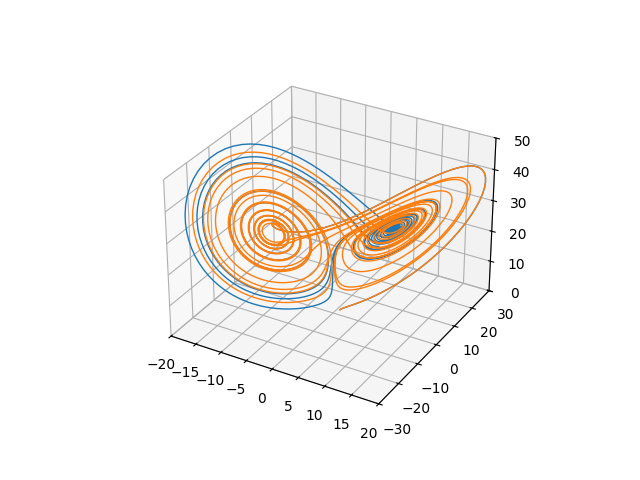
\includegraphics[width=0.9\textwidth]{img/Figure_1.png}
    \caption{Lorenz chaotic phenomena}
    \label{fig:4}
\end{figure}
\newpage
\subsection{Solutions of the Lorenz System Across Various $\rho$ Values}
In the second scenario, we explored the lorenz solution for various values of $\rho$, namely $\rho = [13, 14, 15, 28]$. We observed that for small $\rho$ values, the system exhibited stability and evolved towards one of two fixed-point attractors. However, when $\rho = 28$, these fixed points transformed into repulsors, causing the trajectory to be repelled by them in a highly intricate manner \reff{fig:8}).
\begin{figure}[H]
    \centering
    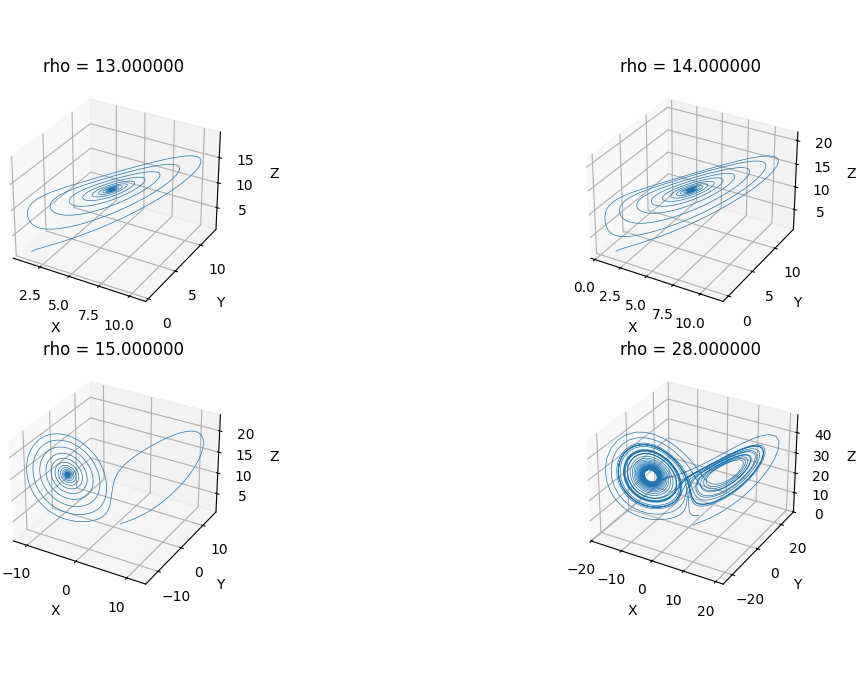
\includegraphics[width=1.\textwidth]{img/lorenz_rho.png}
    \caption{Solutions of the Lorenz System Across Various $\rho$ Values}
    \label{fig:8}
\end{figure}
\newpage
\subsection{Convergence check for Parareal algorithm on lorenz system}
In our third experiment, we utilized the simple Lorenz model with parameter values \(\sigma = 10\), \(b = 8/3\), and \(\rho = 28\), with an initial condition of \(u_0=[1, 1, 1]\). Employing the backward Euler method as both the coarse and fine functions, we established a reference solution with \(10^4\) time steps. We then varied the number of time steps and evaluated the convergence.

Our findings revealed that the error decreased as the number of time steps increased, indicating convergence. (see \reff{fig:5}).
\begin{figure}[ht!]
    \centering
    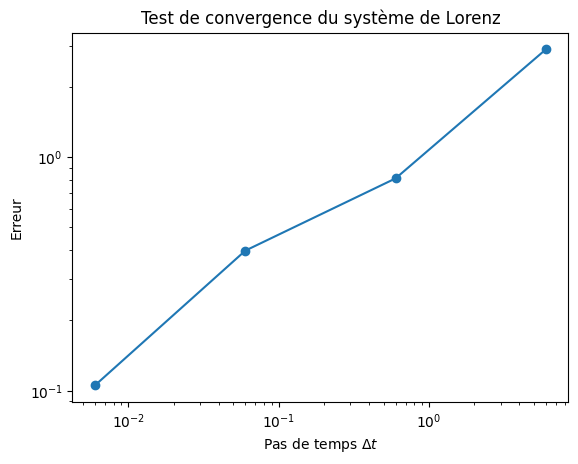
\includegraphics[width=0.78\textwidth]{img/cv.png}
    \caption{Convergence check}
    \label{fig:5}
\end{figure}
\newpage
\subsection{Parareal performance comparison by the number of process}
In our fourth scenario, we employed the simple Lorenz model with parameter values \(\sigma = 10\), \(b = 8/3\), and \(\rho = 28\), along with an initial condition of \(u_0=[1, 1, 1]\). We utilized the explicit Euler method as the coarse function (with one step) and the explicit Euler method (with 100 steps) as the fine function. A reference solution was obtained with \(10^4\) time steps. We varied the number of processes and recorded the processing time.

Our observations revealed that the processing time decreased as the number of processes increased, indicating improved efficiency (see \reff{fig:6}).
\begin{figure}[ht!]
    \centering
    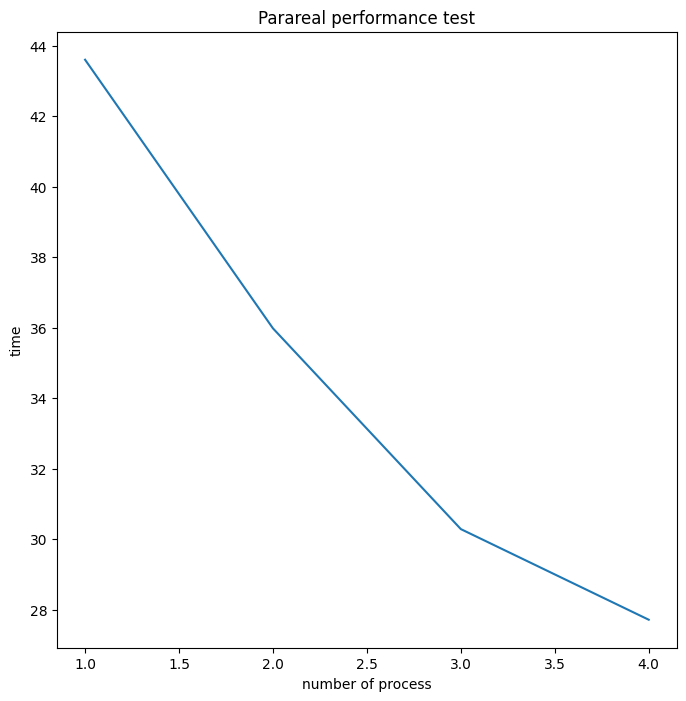
\includegraphics[width=0.7\textwidth]{img/par.png}
    \caption{Parareal performance comparison by the number of process}
    \label{fig:6}
\end{figure}

\newpage

\subsection{Influence of Solver Choice on Parareal Convergence Order}
In the fifth test scenario, we considered a simple ODE $$\frac{dy}{dt} = -t * y^2$$
for which the exact solution is known. We performed two Parareal algorithm implementations:

\begin{enumerate}
    \item Using the implicit Euler method for both the coarse and fine functions.
    \item Using the RK23 and RK45 methods from \texttt{solve\_ivp} for the coarse and fine functions, respectively.
\end{enumerate}
Our observations indicated that the choice of solvers significantly influenced the convergence order. For the first implementation (implicit Euler), we obtained a convergence order of 1.40, whereas the second implementation (RK23 and RK45) yielded a convergence order of 5.38 (see \reff{fig:9}).

\begin{figure}[ht!]
    \centering
    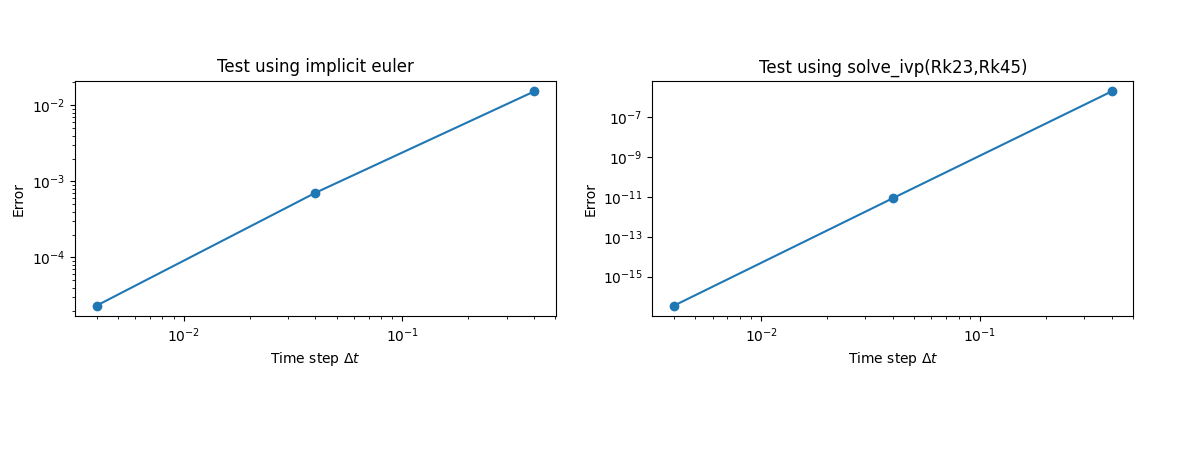
\includegraphics[width=1\textwidth]{img/order_converge.png}
    \caption{Influence of Solver Choice on Parareal Convergence Order}
    \label{fig:9}
\end{figure}
   

%\subsubsection*{Implementation}
%
%We implement the adaptive RK4 (see \reff{fig:4}) method in python.
%
%\begin{figure}[ht!]
%    \centering
%    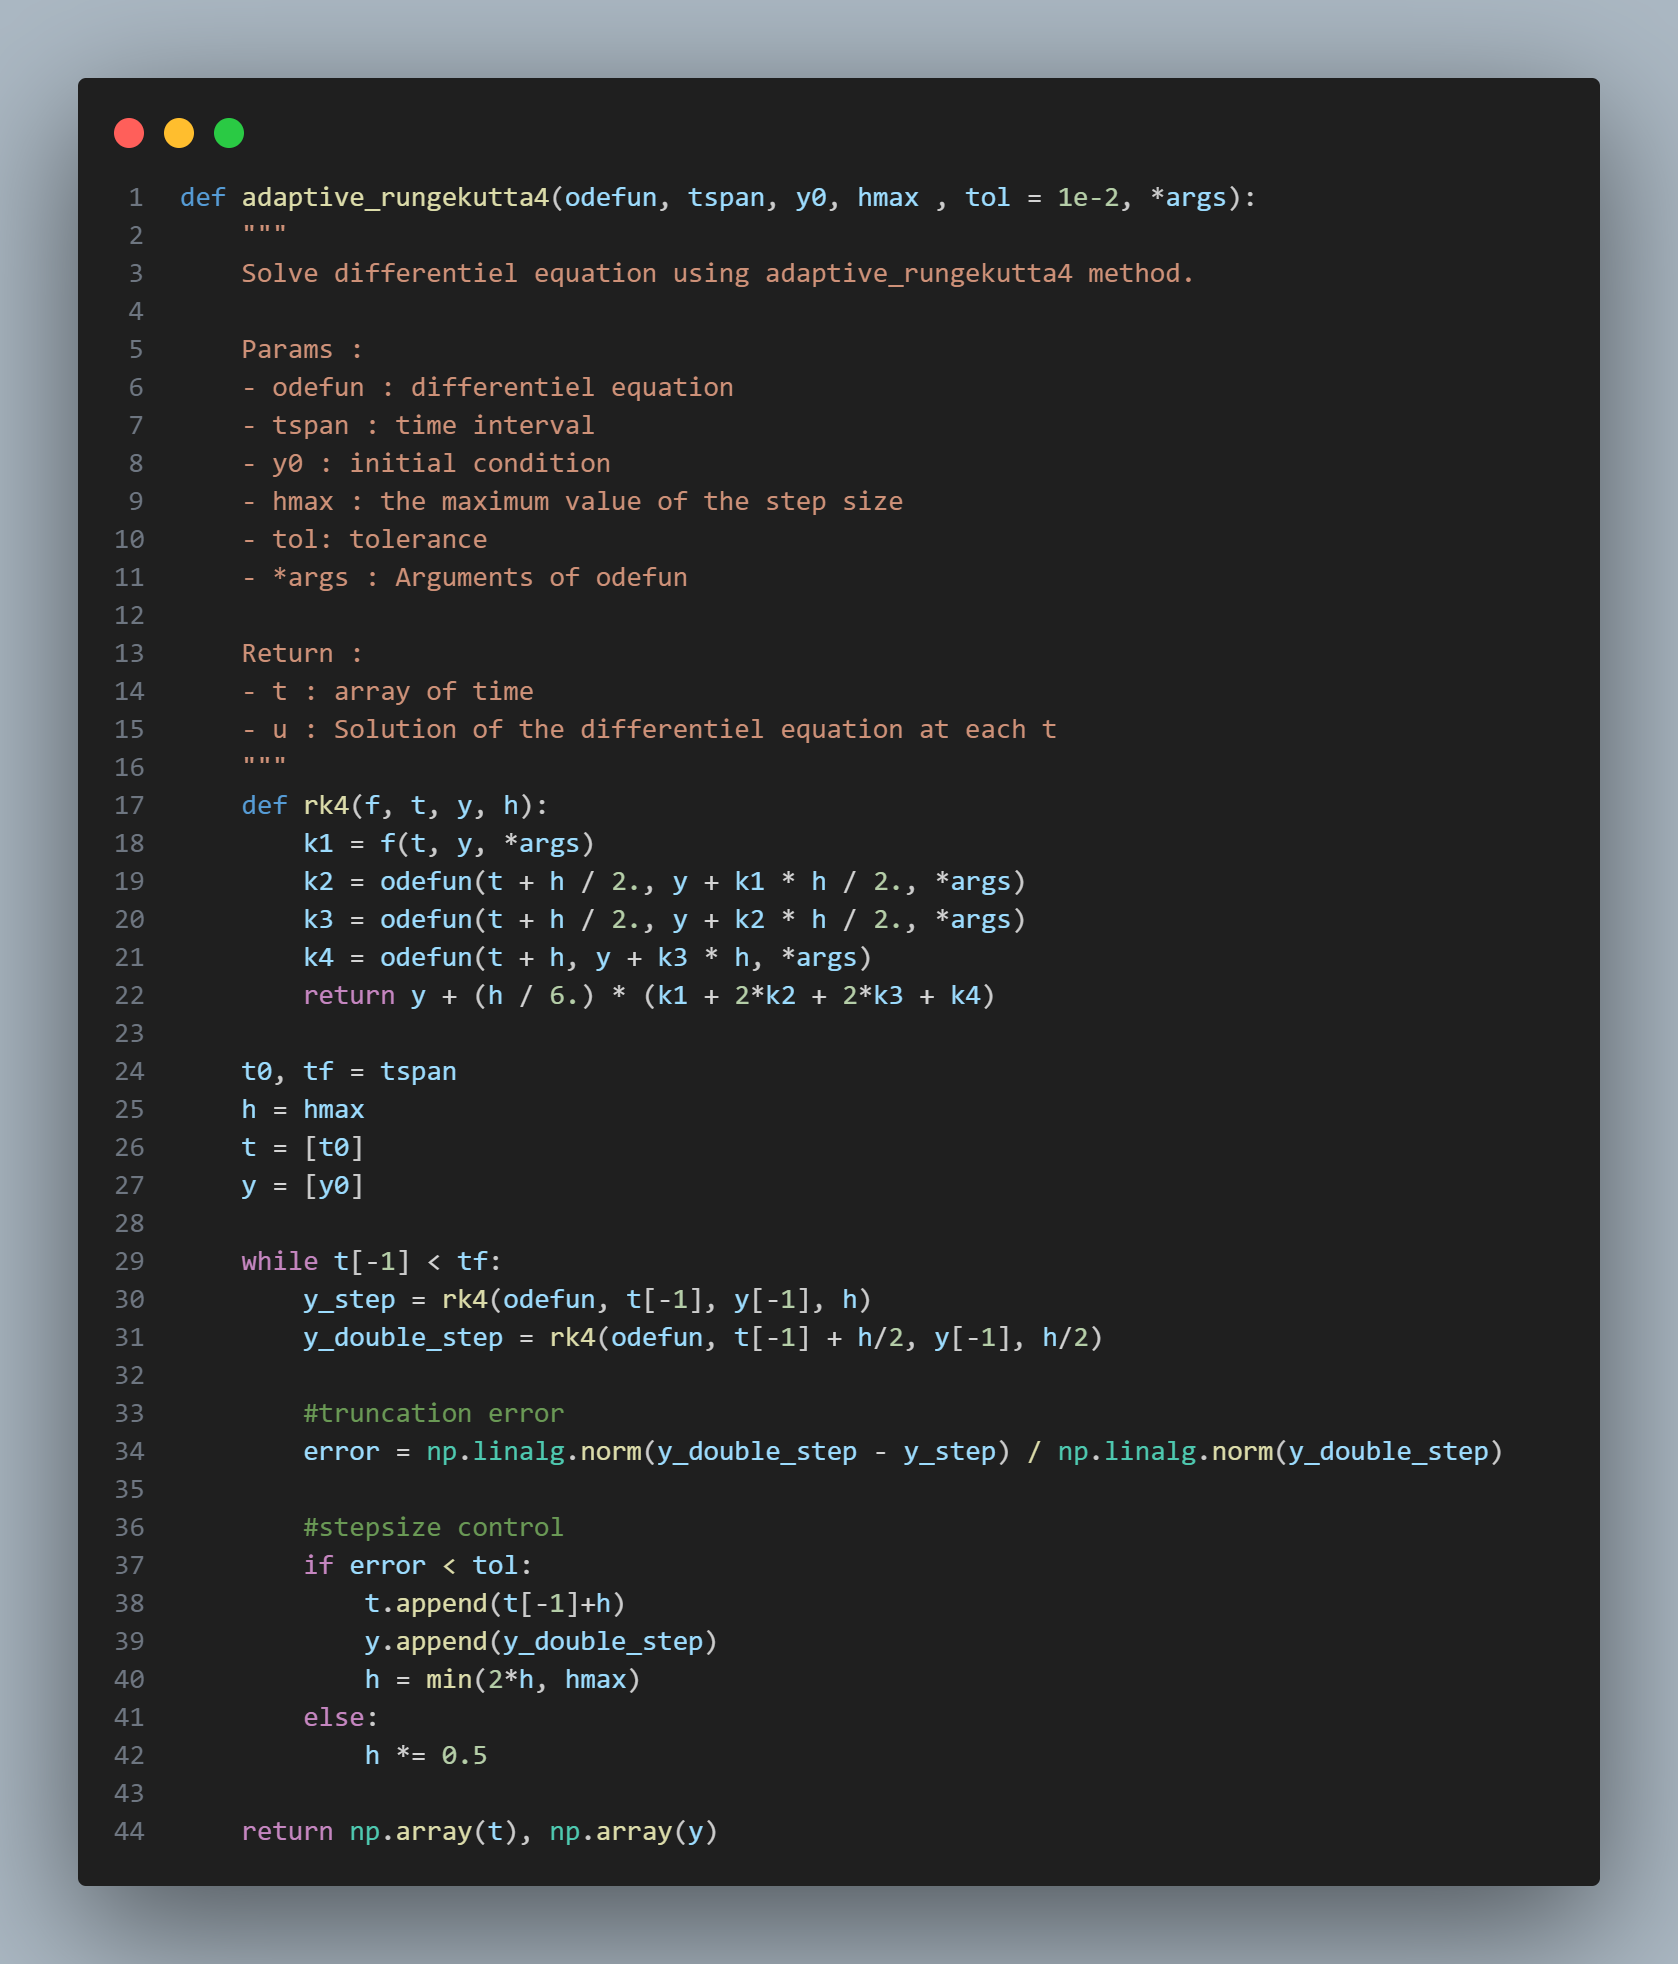
\includegraphics[width=0.78\textwidth]{img/adaptative_rk4.png}
%    \caption{Adaptive RK4}
%    \label{fig:4}
%\end{figure}




% --------------------------------------------------------------
%                            Conclusion
% --------------------------------------------------------------
\newpage
\section{Conclusion}

Each ODE-solving method discussed in this report possesses unique strengths, weaknesses, and applicability in different scenarios. Methods such as Euler, Runge-Kutta, odeint, and \texttt{solve\_ivp} are sequential approaches suitable for a wide range of problems.\\

However, the Parareal algorithm stands out due to its capability to reduce computation time through parallel computing, making it particularly appealing for problems necessitating high precision over extended time intervals. The selection of the method should be guided by the specific requirements regarding precision, computational speed, and implementation complexity of the problem at hand.\\

Furthermore, there's potential for deeper exploration by leveraging the advantages of parallel computing offered by Parareal and integrating it with frameworks like feel++ for solving PDEs in the future. This integration could enhance efficiency and scalability in tackling complex problems in various scientific and engineering domains

\newpage
% --- Biblio par .bib
\bibliography{ref.bib}
\vspace*{\fill}
%\selectlanguage{french}

%\begin{thebibliography}{7}
%\bibitem[Bastien 2019]{id-de-la-source}
%Auteurs : \emph{Un titre},  une date.
%\end{thebibliography}


\end{document}
